\chapter{space game reenactment society}
\label{sec:recreation}
\lhead[tempest]{}
\lstset{style=6502Style}

It was called \textit{ALIEN SPACE GAME}. It didn't test well. It was meant to be a kind of
three-dimensional space invaders knock-off, if we can imagine what that might look like. And we definitely shouldn't.

According to Theuerer: "The initial gameplay was to be simply a ‘First Person Space Invaders’. I got it up and running, but it wasn’t much fun. Too much like Space Invaders (surprise surprise). So after the review they said do you want to kill it? Or have you got any other ideas?"

He did have another idea, it was \textit{Tempest}, so he made that instead. But as we saw in 
\hyperref[sec:things_hidden]{\textcolor{blue}{'things hidden'}}
there is just enough wreckage of that initial concept in the source code for us to imagine what
that first attempt at a game might have looked like.

Scattered here and there we find traces of the crime.

\begin{lstlisting}
SPACG=0			;SUPPRESS SPACE GAME CODE
\end{lstlisting}

Well I'm sorry but the \icode{SPACE GAME} refuses to be fully suppressed. We have already seen some of the intriguing
enemies defined in \icode{ALVROM.MAC}. 

But there are other remnants to be found in there. We find the player's bullets:

\begin{figure}[H]
  \centering
        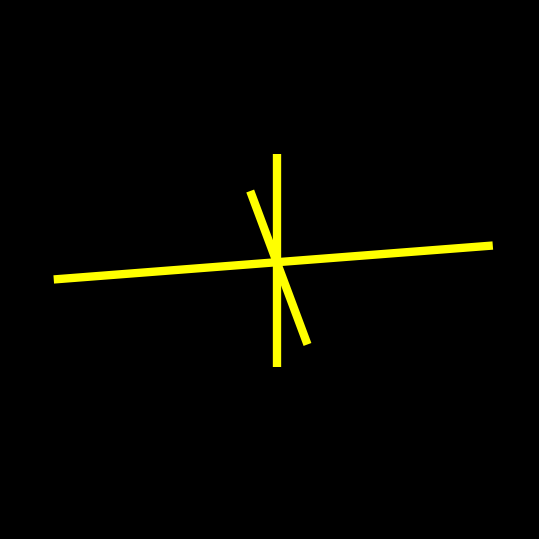
\includegraphics[width=2.22cm]{src/recreation/DSHTBL.png}%
        \hspace{0.2cm}
        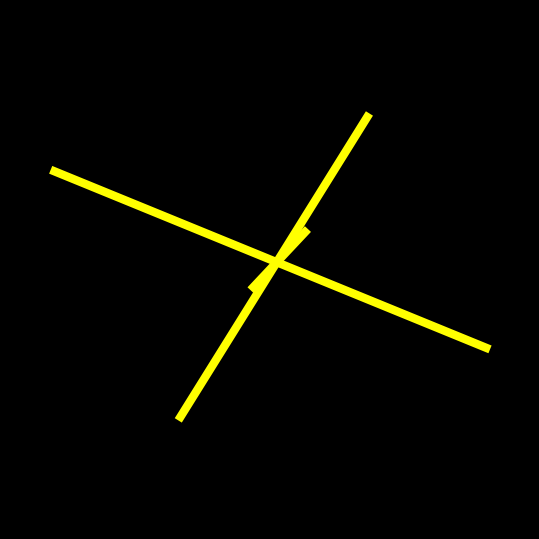
\includegraphics[width=2.22cm]{src/recreation/DS2TBL.png}%
        \hspace{0.2cm}
        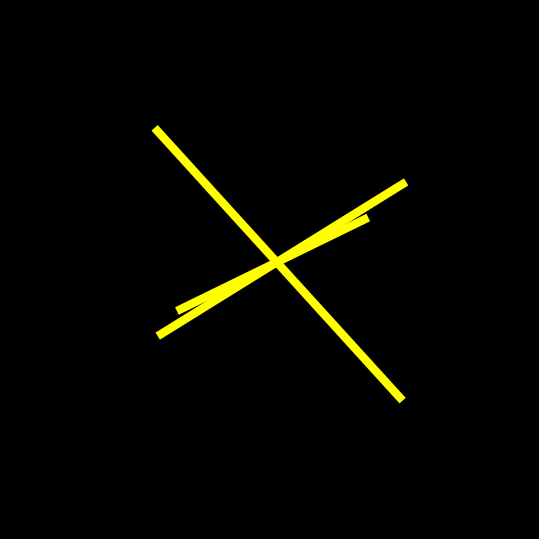
\includegraphics[width=2.22cm]{src/recreation/DS3TBL.png}%
        \hspace{0.2cm}
        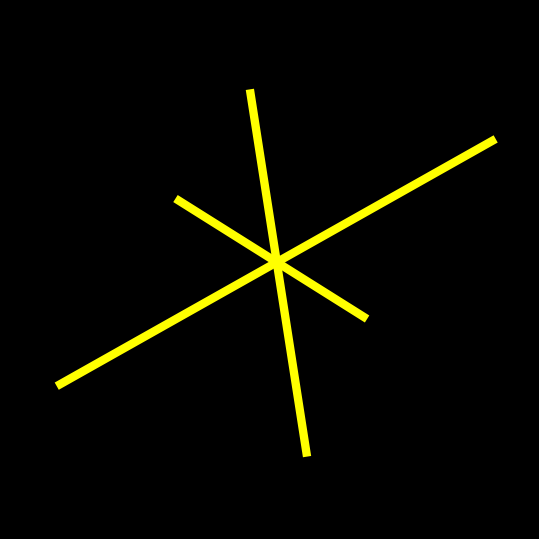
\includegraphics[width=2.22cm]{src/recreation/DS4TBL.png}%
        \hspace{0.2cm}
  \caption*{\icode{DSHTBL}, \icode{DS2TBL}, \icode{DS3TBL} and \icode{DS4TBL} in \icode{ALVROM.MAC}.}
\end{figure}
And the 'spears' fired by the player's enemies:

\begin{figure}[H]
  \centering
        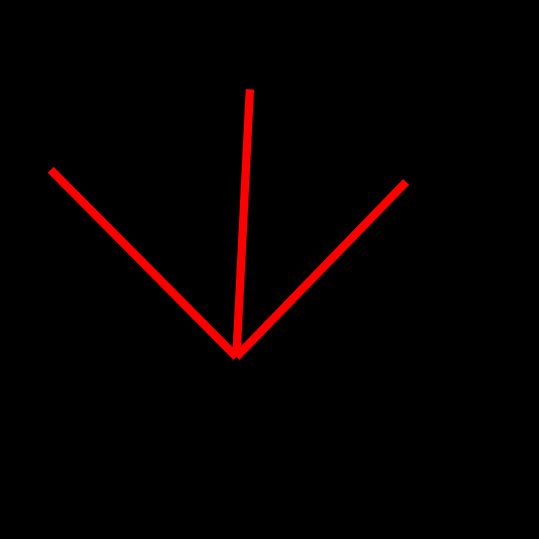
\includegraphics[width=2.22cm]{src/recreation/ESHTBL.png}%
        \hspace{0.2cm}
        
\includegraphics[width=2.22cm]{src/recreation/ES2TBL.png}%
        \hspace{0.2cm}
        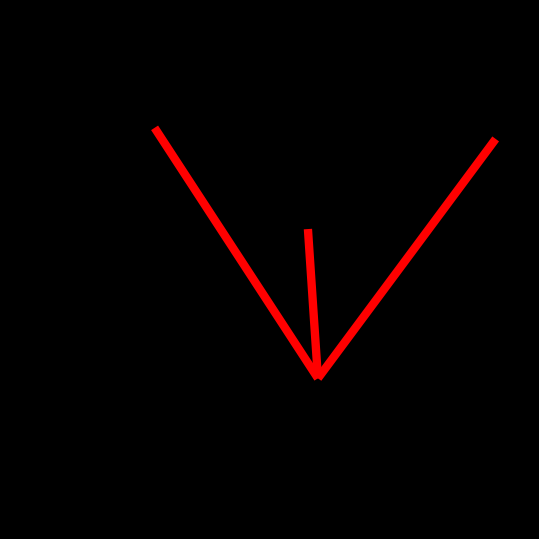
\includegraphics[width=2.22cm]{src/recreation/ES3TBL.png}%
        \hspace{0.2cm}
        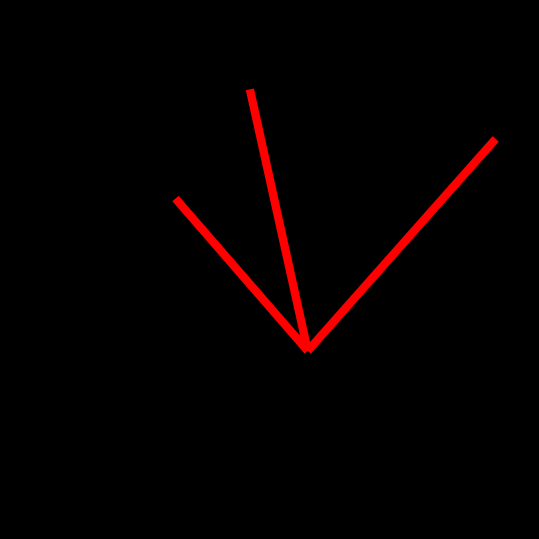
\includegraphics[width=2.22cm]{src/recreation/ES4TBL.png}%
        \hspace{0.2cm}
  \caption*{\icode{ESHTBL}, \icode{ES2TBL}, \icode{ES3TBL} and \icode{ES4TBL} in \icode{ALVROM.MAC}.}
\end{figure}
There is also an 'asteroid', which appears to have been some kind of bomb to be deployed when necessary.

\begin{minipage}[c]{0.48\linewidth}
\begin{figure}[H]
    \centering
    \begin{adjustbox}{width=4.5cm,center}
        
\includegraphics[width=5cm]{src/recreation/asteroid.png}%
    \end{adjustbox}
  \caption*{\icode{ASTTBL} in \icode{ALVROM.MAC}.}
\end{figure}
\end{minipage}
\begin{minipage}[c]{0.48\linewidth}
\begin{lstlisting}
ASTTBL: .BYTE ENDAST-ASTTBL
        .BYTE -6,0,0
        .BYTE 3,5,4
        .BYTE 3,5,-4
        .BYTE 0,-5,0
\end{lstlisting}
\vspace*{\fill}
\end{minipage}

We find the definition of a primitive-looking 'fort', a simple pyramid shape that perhaps served as
an obstacle that the player could hide behind to avoid enemy 'spears' and which was perhaps eventually
degraded by enemy attack over time.  To draw the forts a macro called \icode{FORTMAC} was used to draw
the same pyramidal shape with the initial dimension specified as a parameter \icode{FS}.
\clearpage
\begin{lstlisting}
.MACRO FORTMAC .FS
  VCTR .FS,-<.FS/3>,0
  VCTR -.FS,.FS,6
  VCTR -.FS,-.FS,6
  VCTR 2*.FS,0,6
  VCTR -.FS,<.FS/3>,0
  RTSL
.ENDM
\end{lstlisting}


It appears this degradation was implemented by gradually reducing the
size of the fort - as you can see by the values on the axis on the images below.

\begin{minipage}[c]{0.48\linewidth}
\begin{figure}[H]
    \centering
    \begin{adjustbox}{width=5.5cm,center}
        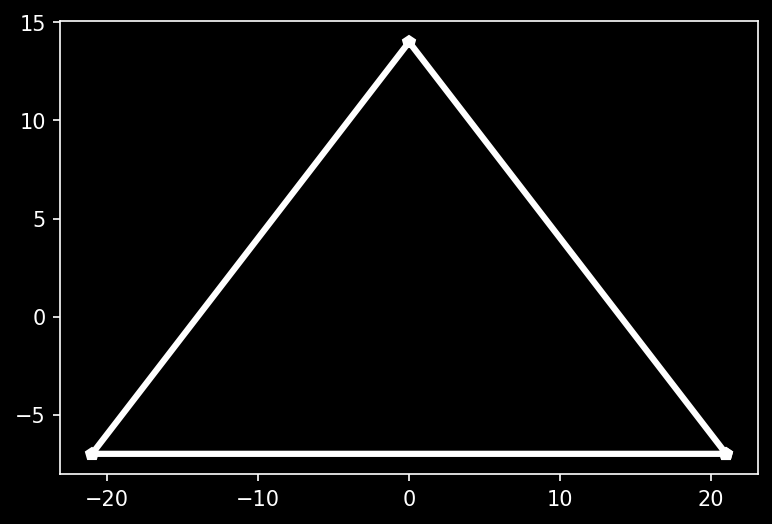
\includegraphics[width=5cm]{src/recreation/FORT1.png}%
    \end{adjustbox}
  \caption*{\icode{FORTMAC 15} in \icode{ALVROM.MAC}.}
\end{figure}
\end{minipage}
\begin{minipage}[c]{0.48\linewidth}
\begin{figure}[H]
    \centering
    \begin{adjustbox}{width=5.5cm,center}
        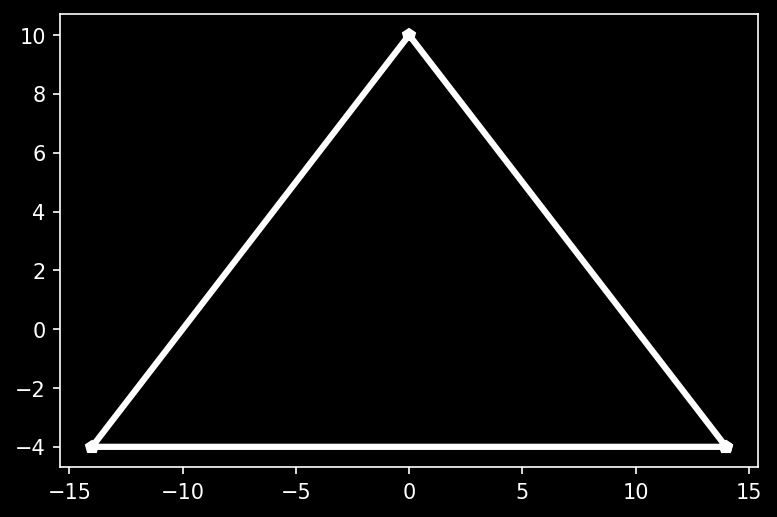
\includegraphics[width=5cm]{src/recreation/FORT3.png}%
    \end{adjustbox}
  \caption*{\icode{FORTMAC 10} in \icode{ALVROM.MAC}.}
\end{figure}
\end{minipage}

\begin{minipage}[c]{0.48\linewidth}
\begin{figure}[H]
    \centering
    \begin{adjustbox}{width=5.5cm,center}
        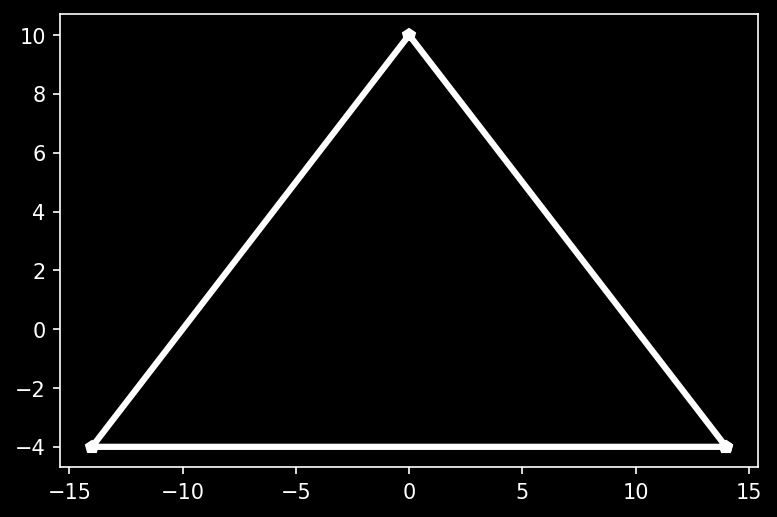
\includegraphics[width=5cm]{src/recreation/FORT3.png}%
    \end{adjustbox}
  \caption*{\icode{FORTMAC 0E} in \icode{ALVROM.MAC}.}
\end{figure}
\end{minipage}
\begin{minipage}[c]{0.48\linewidth}
\begin{figure}[H]
    \centering
    \begin{adjustbox}{width=5.5cm,center}
        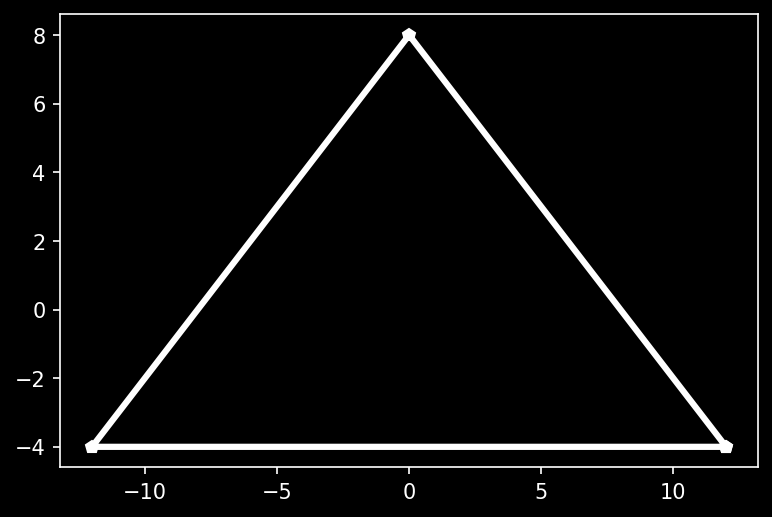
\includegraphics[width=5cm]{src/recreation/FORT4.png}%
    \end{adjustbox}
  \caption*{\icode{FORTMAC 0C} in \icode{ALVROM.MAC}.}
\end{figure}
\end{minipage}

Finally we find the remains of the player's ship. Unfortunately it is something of a disappointment - so clearly little
more than a placeholder.

\begin{minipage}[c]{0.48\linewidth}
\begin{figure}[H]
    \centering
    \begin{adjustbox}{width=4.5cm,center}
        
\includegraphics[width=5cm]{src/recreation/GUN.png}%
    \end{adjustbox}
  \caption*{\icode{GUNPIC} in \icode{ALVROM.MAC}.}
\end{figure}
\end{minipage}
\begin{minipage}[c]{0.48\linewidth}
\begin{lstlisting}
GUNPIC: VCTR -8,0,6
        VCTR -8,-10,6
        VCTR -10,0,6
        VCTR -8,-18,6
        VCTR 50,0,0
        VCTR -8,18,6
        VCTR -10,0,6
        VCTR -8,10,6
        VCTR -8,0,6
        RTSL
\end{lstlisting}
\vspace*{\fill}
\end{minipage}

There are other clues. We find the remnants of what must have been the game's playefield, a grid-like
structure. which despite its name contain 10 vertical lines rather than just 5.
\begin{lstlisting}
        .SBTTL DRAW TABLES:GRID LINES
VRT4DRW:
VRT5DRW:                        ;DRAW 5 VERT LINES
        TLABS 0
        SBRITE 040
        TVCTR 1
        SBRITE 0
        TVCTR 3
        SBRITE 040
        TVCTR 2
        SBRITE 0
        TVCTR 4
        SBRITE 040
        TVCTR 5
        SBRITE 0
        TVCTR 7
        SBRITE 040
        TVCTR 6
        SBRITE 0
        TVCTR 8
        SBRITE 040
        TVCTR 9
        OBJEND
\end{lstlisting}
If we put all these elements together we can make a wild and unfounded speculation as to how
\textit{ALIEN SPACE GAME} might have looked. 

\begin{figure}[H]
  \centering
        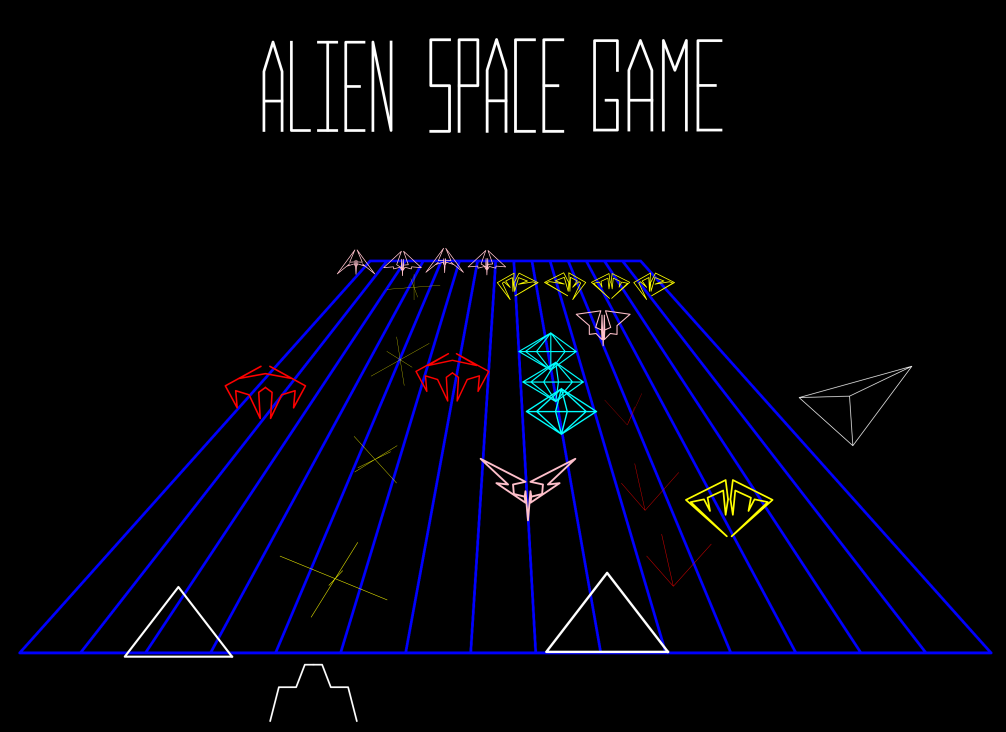
\includegraphics[width=13cm]{src/recreation/recreation-1.png}%
  \caption*{I probably shouldn't have even tried.}
\end{figure}

This is my deeply wonky attempt at visualising such
a thing. Note that I've assumed that 'first person' space invaders must involve some kind of version
of the classic space invaders playfield but with a three-dimensional depth of field: the baddies come
at us slowly from the back of the screen, getting larger as they approach. Our player sits at the near
edge of the field shooting along the grid that the enemies advance across. The 'forts' sit in front of the
player and presumably can shield him from enemy attack. Meanwhile the asteroid is hanging out there in
space in search of a purpose. Aren't we all, darling.

